
\documentclass[11pt, a4paper]{article}
\usepackage[left=1.5cm,text={18cm, 25cm},top=2cm]{geometry}
\usepackage[T1]{fontenc}
\usepackage[bf]{caption}
\usepackage{hyperref}
\usepackage[all]{hypcap}
\usepackage[utf8]{inputenc}
\usepackage{graphicx}
\usepackage[czech, english]{babel}
\selectlanguage{english}
\usepackage{subfig}                % \subfloat
\usepackage{color}
\usepackage{url}
\inputencoding{utf8}
%\usepackage[bf]{caption2}
\usepackage{hyperref}
\usepackage[all]{hypcap}
\hypersetup{colorlinks=false, linkbordercolor=1 1 1, citebordercolor=1 1 1}
\usepackage[right]{lineno}
\usepackage{listings}
\renewcommand\linenumberfont{\normalfont\tiny\color{blue}}

% Theming listing
\definecolor{commentsColor}{rgb}{0.497495, 0.497587, 0.497464}
\definecolor{keywordsColor}{rgb}{0.000000, 0.000000, 0.635294}
\definecolor{stringColor}{rgb}{0.558215, 0.000000, 0.135316}

\lstset{ %
    commentstyle=\color{commentsColor},
    keywordstyle=\color{keywordsColor},
    numberstyle=\color{commentsColor},
    rulecolor=\color{black},
    stringstyle=\color{stringColor},
}


\iflanguage{english}{
    \renewcommand{\uv}[1]{``#1''}
}

\title{Visualization of SDF scenes}
\author{Petr Fusek <xfusek08@stud.fit.vutbr.cz>}
\date{\today}


%--------------------------------------------------------------------------------


\begin{document}
\selectlanguage{english}
\maketitle

\section{Introduction}

This semester project is developed as a shared project for two classes: \uv{GMU - Graphic and Multimedia Processors} and \uv{PGPa - Advanced Computer Graphics}.
As a~disclaimer, it should be noted that this project is still a~work in progress and its final goal is beyond the scope of one semester's work. It will be improved and built upon in my upcoming master's thesis.
Therefore, the results achieved thus far are more of a!\uv{proof of concept} rather than a~finished, self-contained work.

\subsection{Motivation}

The final goal of the upcoming thesis is to develop a~simple, user-friendly 3D sculpting application using a~non-traditional technique for storing and rendering 3D models developed by \emph{Media Molecule} \footnote{\href{https://www.mediamolecule.com/}{https://www.mediamolecule.com/}} for its game \emph{Dreams}{\texttrademark}.
This game engine is accessible to unexperienced, non-technical users and allows for the creation of highly detailed 3D models and scenes without worrying about polygon counts, texturing, or levels of detail.

This project is based on my research of the basic principles of this technology and the possible implementation of a~simplified version for PC users.

\subsection{Goals}

To stay within the scope of the two classes, the aim of this work will be a~GPU-based evaluator (for GMU) and a~3D renderer of the resulting representation (for PGPa).
The basic idea is to have the geometry of a~3D model represented by \emph{Constructive Solid Geometry} (CSG) of a~small set of basic primitive shapes, which will be evaluated into a \emph{Signed Distance Field}. This field will be rendered onto the screen using an optimized \emph{rasterization pipeline} on the GPU.

%%%%%%%%%%%%%%%%%%%%%%%%%%%%%%%%%%%%%%%%%%%%%%%%%%%%%%%%%%%%%%%%%%%%%%%%%%%%%%%%%%%%%%%%

\section{Theory}

The main source of this technology is a talk given by Alex Evans \cite{evans2015} about the technology used by Media Molecule in \emph{Dreams}{\texttrademark}.

\subsection{Scene representation}

The rendered scene is composed of \emph{geometries} and \emph{models}.
Models in their core are an instance of a~geometry positioned in world space with some potential shading data.
Geometries can be shared by objects and are composed of list of \emph{edits}.
Edits are added into a~list and each represents some incremental change to overall geometry.
Changes are mostly additions and subtractions of some primitive volumetric shapes creating a~simplified (entirely lef-leaning) CSG tree.
Edit lists needs to be evaluated into a~renderable data structure which is job of the \emph{evaluator}.

This whole structure has several reasons.
3D sculpting by incrementally adding and subtracting volumes is more intuitive for the user.
Resulting edit list is convenient compact representation of geometry (In theory just tents of KB for big detailed models.).
And it is directly easily rendderable as composed \emph{Signed Distance Function} (SDF) by \emph{ray-marching}/\emph{sphere-tracing}, which is a~popular technique used by pixel-shader programmers of \emph{Shadertoy}\footnote{\href{www.shadertoy.com}{www.shadertoy.com}} community.
This has another advantage of implicitly representing smooth surfaces (see figure \ref{ray_marching_fig}).
\begin{figure}
    \centering
    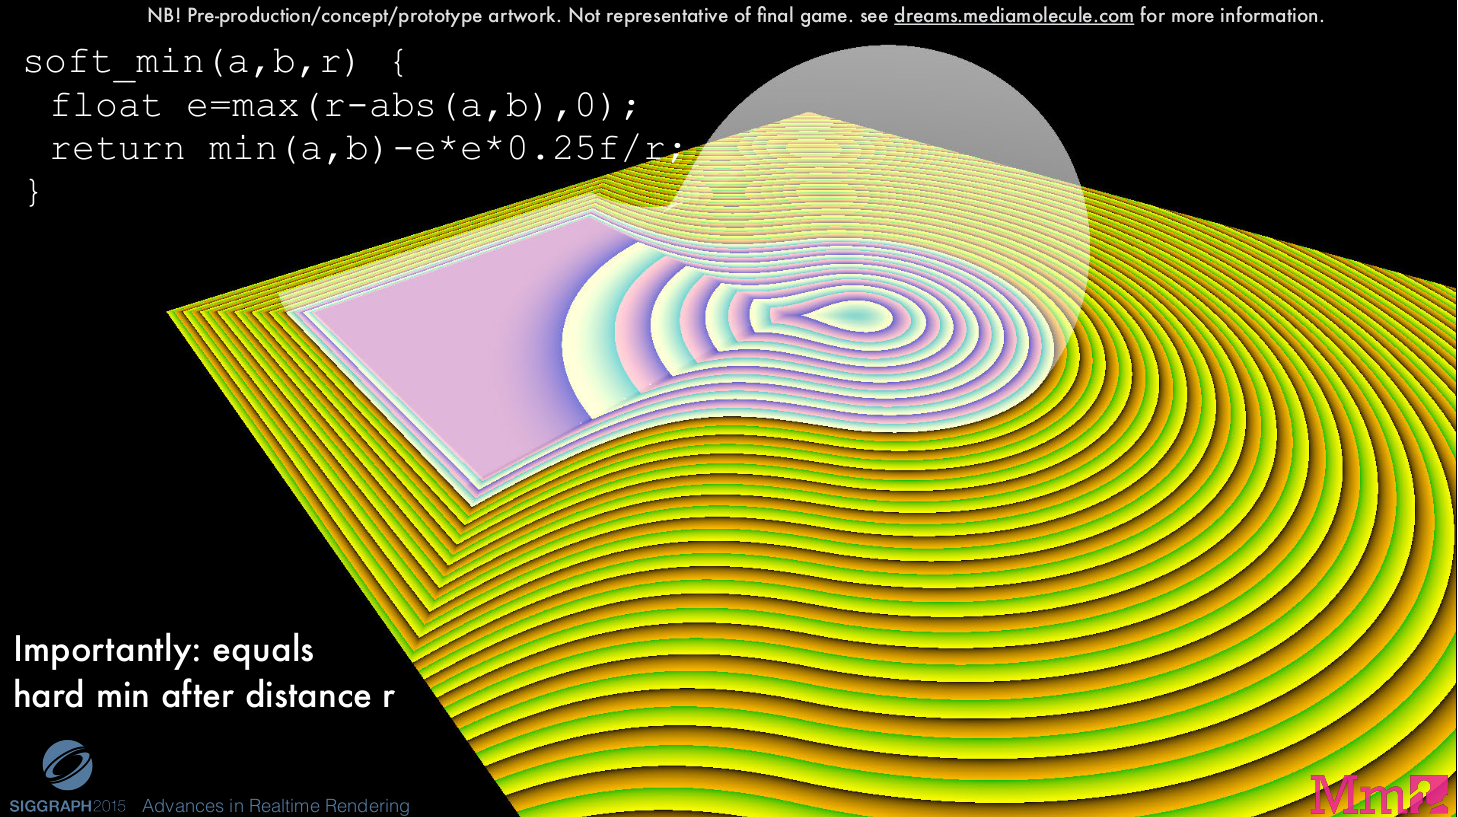
\includegraphics[height=5cm,keepaspectratio]{SDF.png}
    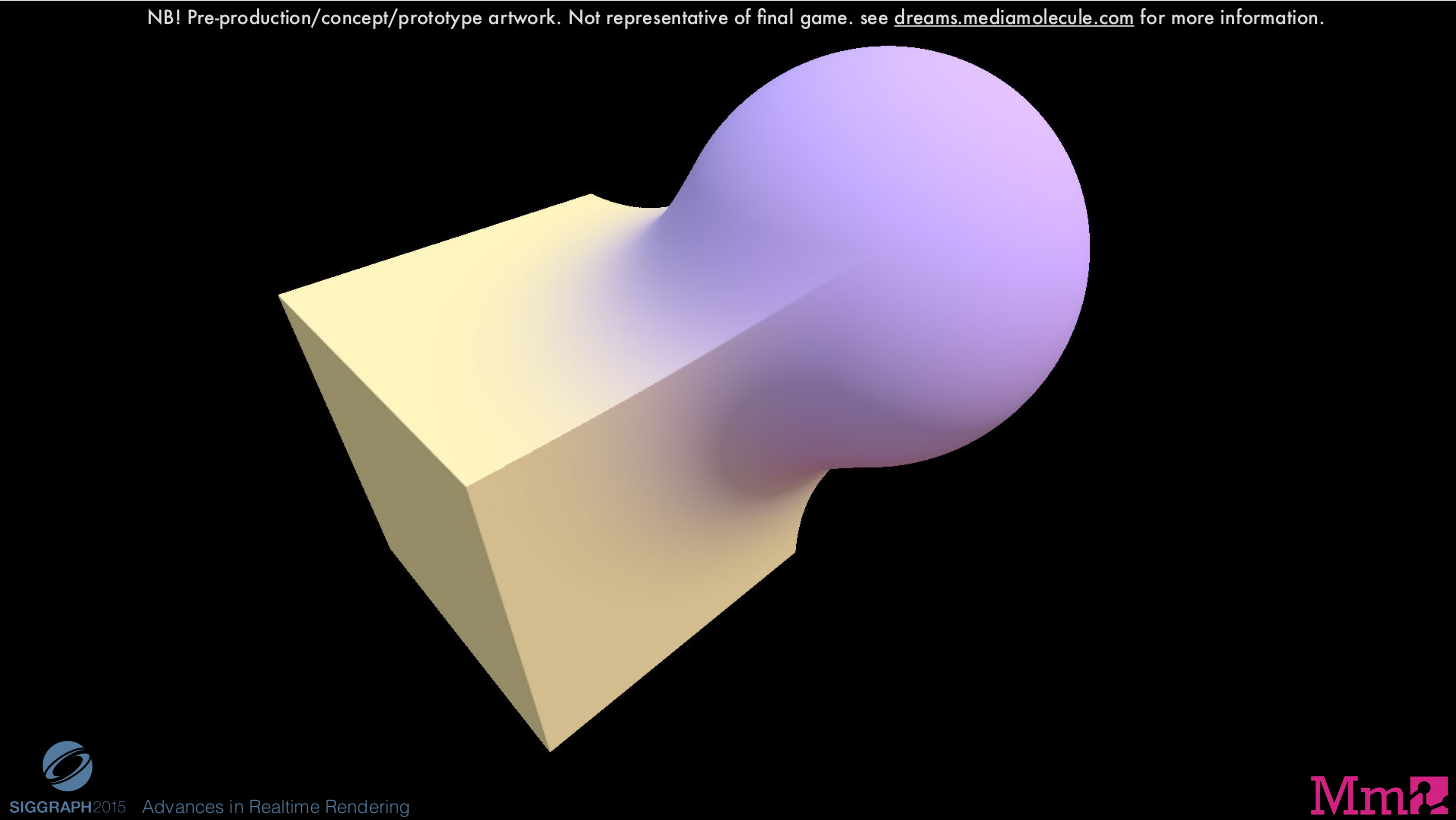
\includegraphics[height=5cm,keepaspectratio]{SDF_RES.png}
    \caption{Left - Visualization of 3D SDF of two edits. Right - Smooth surfaces obtained by sampling the SDF. Images are taken from \cite{evans2015}}
    \label{ray_marching_fig}
\end{figure}

\subsection{Rendering pipeline}

Directly ray-marching whole complex scenes composed of large number of primitives in each pixel of the screen is to slow for real-time applications.
So the whole task for rendering pipeline is to render large number of complex geometries (SDFs) onto screen in real time.
Overview of the pipeline idea is on the figure~\ref{pipeline_idea}.
From the diagram we can see that evaluator will transform list of edit into a~\emph{Sparse Voxel Octree} (SVO) which will be stored in the GPUs memory.
All models are rendered each frame using SVO representation and properties from currently rendered model.

\subsection{Evaluator}
Evaluator uses GPUs compute shader to create an SVO with brick pool into a~GPU memory.
Implementation of SVOs structure is mostly identical to the one used in Crassins Gigavoxels \cite{crassin2011}.
Main two parts of the evaluated geometry are \emph{Node Pool} and \emph{Brick Pool}.
Node Pool is and encoded octree representation stored in linear memory of gpu, where one node is represented by two integers. First one holds pointer to \emph{child node tile} and second points to brick in brick pool. See figure \ref{fig_note_tree}.
\begin{figure}[ht!]
    \centering
    \raisebox{-0.5\height}{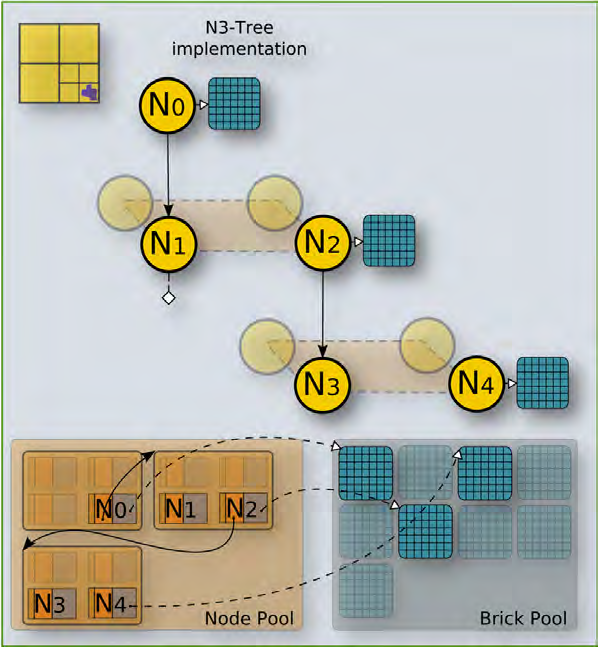
\includegraphics[height=5cm,keepaspectratio]{node_tree.png}}
    \hspace*{.2in}
    \raisebox{-0.5\height}{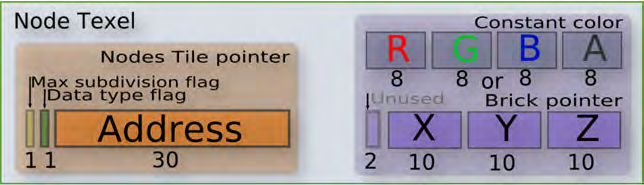
\includegraphics[height=2.5cm,keepaspectratio]{node_texel.png}}
    \caption{
        Sparse voxel octree structure in GPU memory.
        Nodes siblings are stored in tiles to which parent holds and offset pointer.
        Nodes may point to a~brick stored in brick pool implemented using 3D texture atlas.
        Images are taken from \cite{crassin2011}
    }
    \label{fig_note_tree}
\end{figure}

\begin{figure}
    \centering
    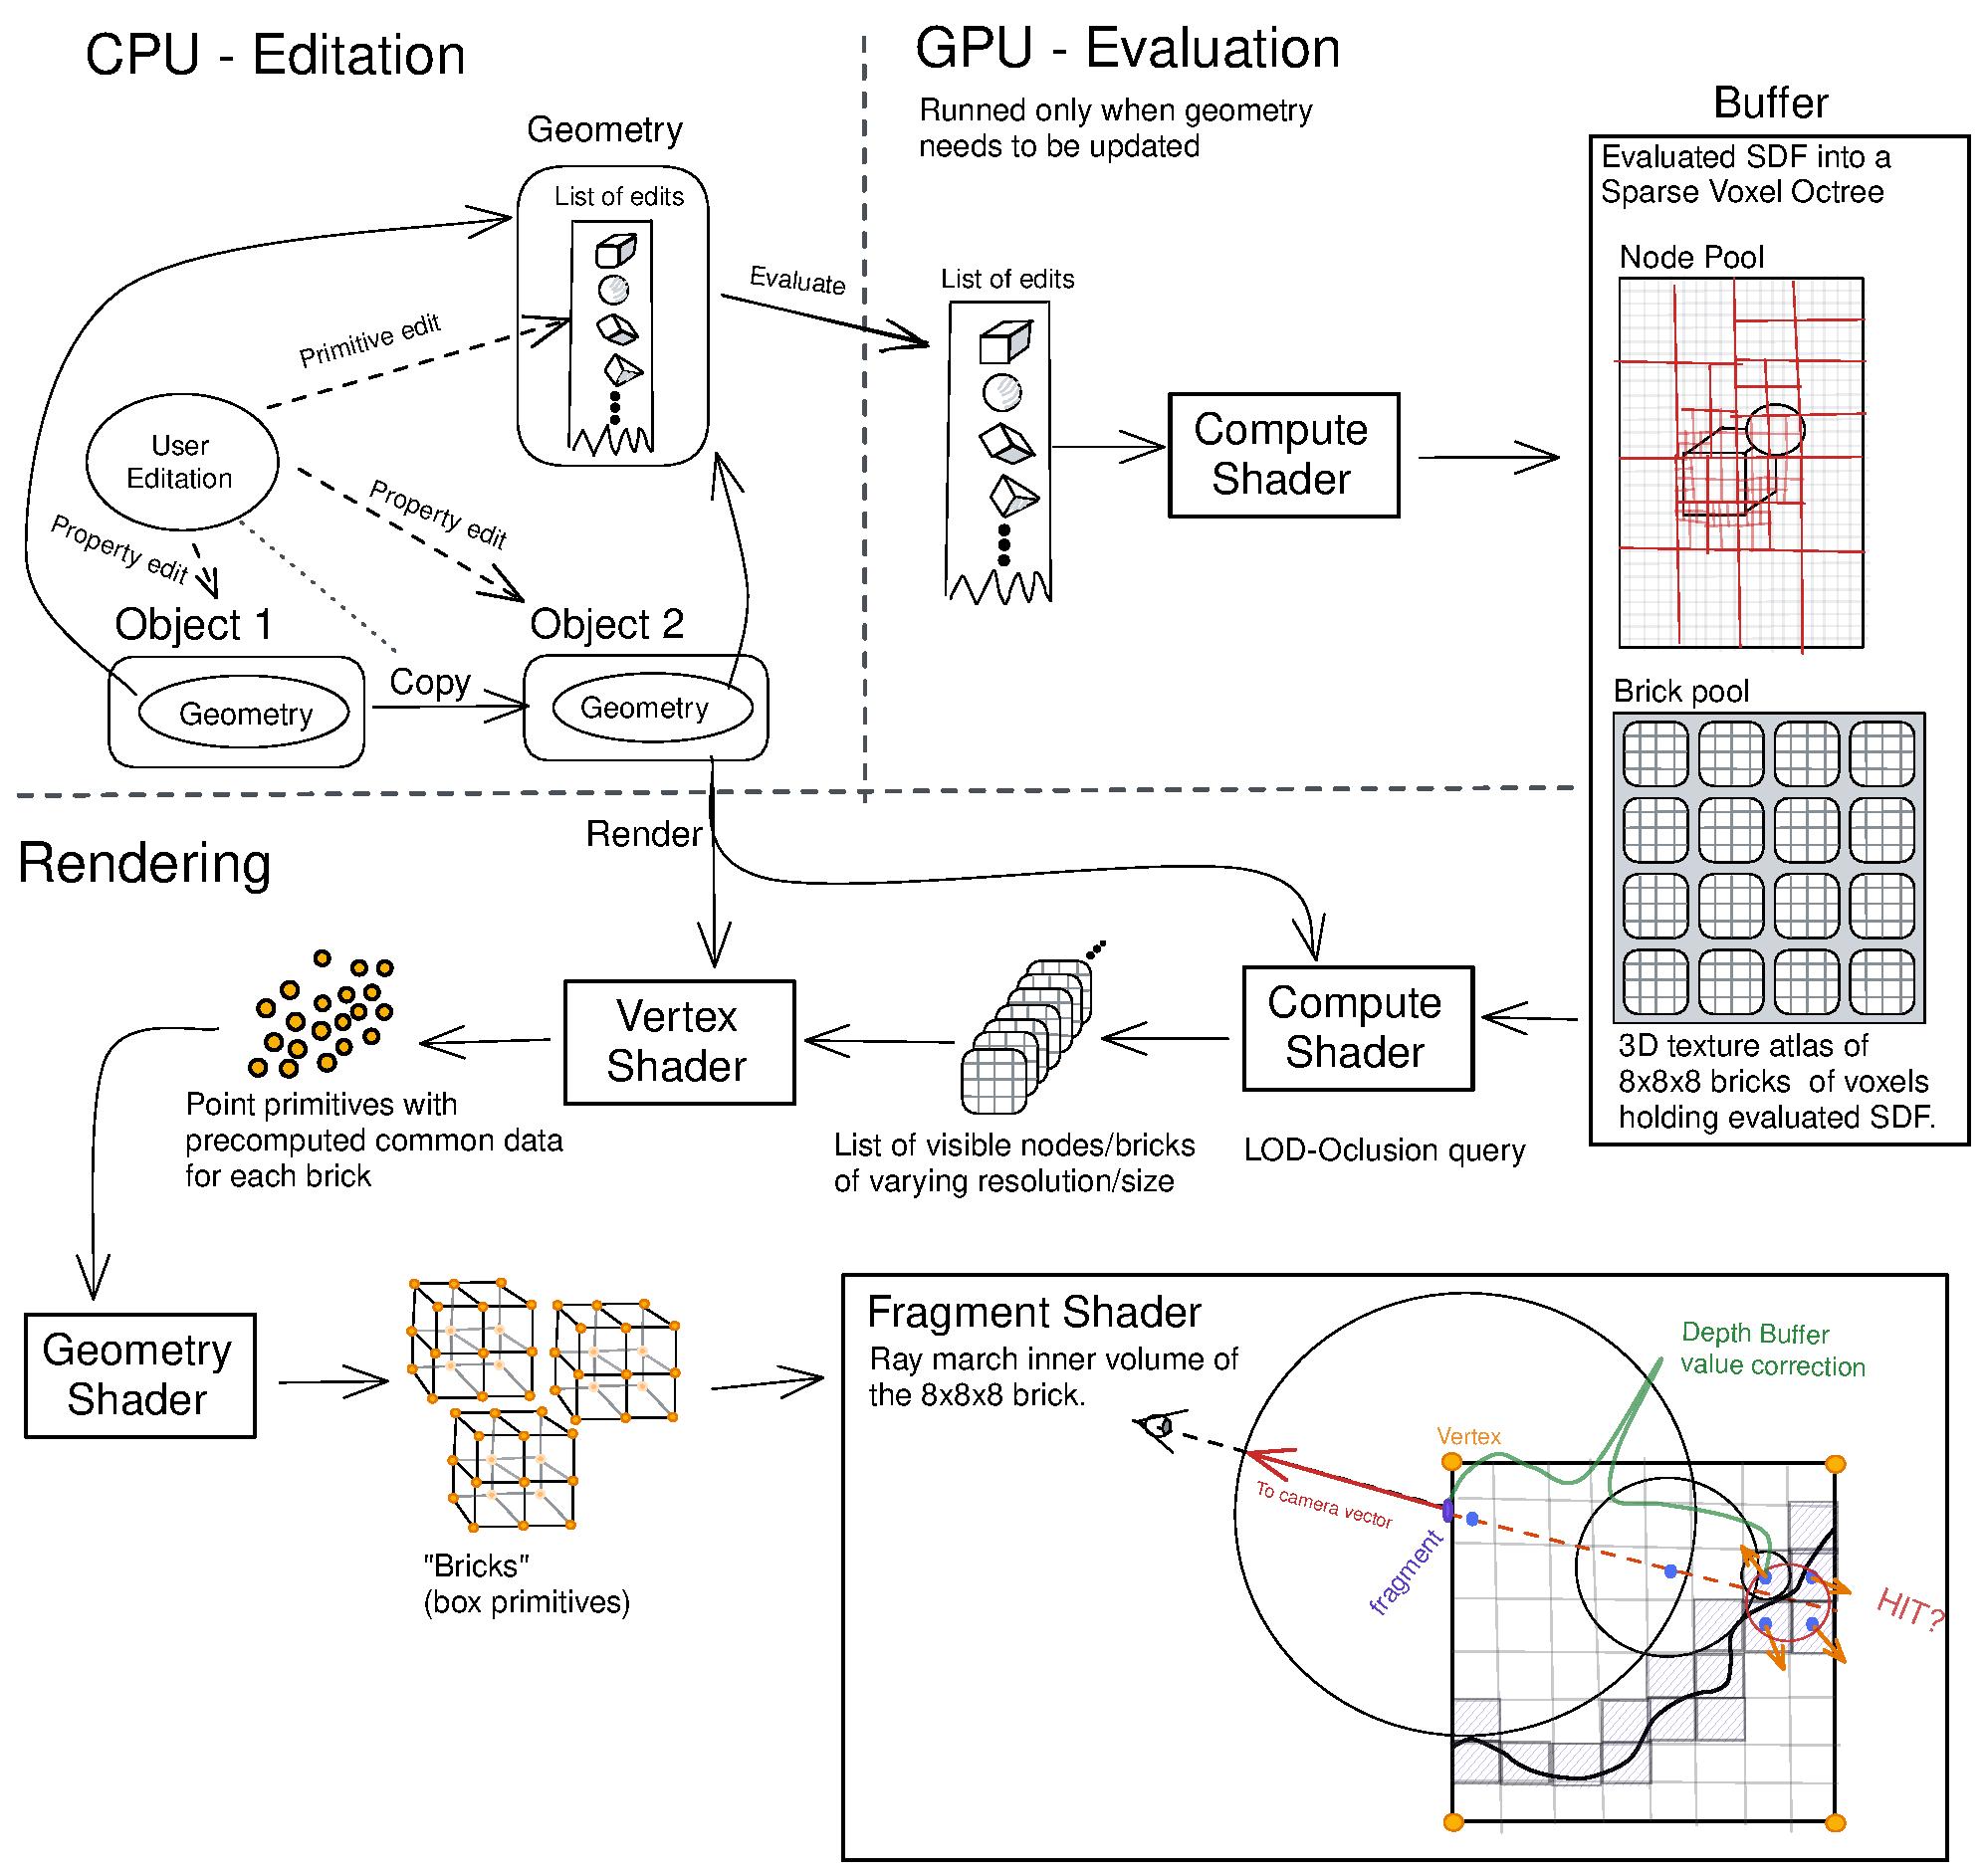
\includegraphics[width=\textwidth]{desing_idea.pdf}
    \caption{Idea of rendering pipeline.}
    \label{pipeline_idea}
\end{figure}

The algorithm for constructing the SVO on octree was inspired by the work in \cite{crassin2012}, but it has been redesigned to suit an SDF evaluation.
The construction is done using a~top-down approach, evaluating one level of the octree in one dispatch. The main rule is that the currently evaluated node will be divided if it intersects with the surface of the geometry, meaning that at least one voxel in the potential node brick has a~distance value smaller than the size of that voxel.
This means that when descending through the levels, all 512 voxels per node-brick need to be sampled, and if there is an intersection, the node is marked to be divided, and the brick is stored in a~brick pool.
Therefore, the algorithm dispatches a~group of 512 threads per node in the currently evaluated level, and each group may spawn a~new tile of 8~nodes for the next level.

\subsection{Rendering}
As can be seen in the diagram \ref{pipeline_idea}, the rendering process uses the evaluated SVO with the brick pool to render bricks of SDF data onto the screen.
The main advantage of this approach is the ability to use filtered LOD and good culling possibilities, as all algorithms work directly with the octree or with a~cloud of cubes in world space.

When rendering a~model, its geometry is transformed to its position, and nodes that hold a~reference to a~brick and are visible on the screen are selected. The result is a~list of integer indices to a~node pool associated with the model, which can be submitted for rendering as a~point cloud.
On the GPU side, the precomputed shading and transformation properties of each index are calculated in the vertex shader.
The geometry shader will spawn a~cube to be rasterized onto the screen in the correct position.
The fragment shader will ray-march from the rasterized surface fragment until it hits the geometry surface or the other side of the cube.
When a~hit is detected, the normal is computed by sampling the gradient of the brick's SDF, and it is used for simple lighting.

%%%%%%%%%%%%%%%%%%%%%%%%%%%%%%%%%%%%%%%%%%%%%%%%%%%%%%%%%%%%%%%%%%%%%%%%%%%%%%%%%%%%%%%%

\section{Implementation}

Project was implemented using a~\texttt{C++20} with CMake\footnote{\href{https://cmake.org/}{www.cmake.org}} using OpenGL 4.6\footnote{\href{https://www.opengl.org/}{www.opengl.org}}, glm\footnote{\href{https://glm.g-truc.net/0.9.9/index.html}{www.glm.g-truc.net/0.9.9/index.html}}, glfw\footnote{\href{https://www.glfw.org/}{www.glfw.org}} libraries.
Used HW was: AMD Ryzen{\scriptsize\texttrademark} 7 5800H\footnote{\href{https://www.amd.com/en/products/apu/amd-ryzen-7-5800h}{www.amd.com/en/products/apu/amd-ryzen-7-5800h}}
with AMD Radeon{\scriptsize\texttrademark} Graphics.
\subsection{Building}
Project was developed and tested on linux under PoP\_OS!\footnote{\href{https://pop.system76.com/}{pop.system76.com}} distribution.
All dependencies should be included in its repository directly or as git submodules.
Projects source code is available on GitHub\footnote{\href{https://github.com/xfusek08/SDFEdit}{github.com/xfusek08/SDFEdit}}.

\subsection{Implementation of evaluator on GPU}
Evaluator was implemented using OpenGLs compute shaders API.
Final algorithm is more or less same as was proposed in theory section.
The final implementation of evaluated geometry is composed of three OpenGL buffers to store octree data and one 3D texture as a~brick atlas as it shown in following pseudo code:
\begin{lstlisting}[language=C++]
struct Octree {
    Buffer<uint> nodes; // pointer to child tile + has-brick/has-child flags
    Buffer<uint> nodeData; // nodes brick coordinates in brick pool
                           // or empty/full flag
    Buffer<vec4> verticies; // (x,y,z) - position of node center in octree space
                            // w - length of brick/nodes edge
    Texture3D<float> brickPool; // of some predefined resoluton N~x N~x N~voxels
}
\end{lstlisting}
By octree space is meant coordinate system where octree of geometry is at the center.

\subsubsection{Algorithm of SVO construction}
On CPU there is implemented a~maximum number of subdivision for the SVO.
There are two shader programs performing two task: \emph{Level evaluator} evaluates SDFs into bricks and alocates space for nodes in next level.
\emph{Level initiator} zeros allocated memory for new nodes and computes verticies for nodes in next level.
Following pseudocode describes cpu side of the algorithm.

\begin{lstlisting}[language=C++]
Program level_evaluator;
Program level_initiator;
AtomicCounter node_count = 8; // 1st tile - 8~uninitialized allocated nodes
int level_start_node = 0;
int level_node_count = node_count;

level_initiator.setLevelStartUniform(level_start_node);
level_initiator.dispatch(1, 8); // 1 group, 8 threads per group
for (i in 0 .. maxSubdivision) {
    level_evaluator.setLevelStartUniform(level_start_node);
    level_evaluator.dispatch(level_node_count, {8, 8, 8}); // 512 threads
    int next_level_start = level_start_node + level_node_count;
    int next_level_node_count = node_count - next_level_start;
    if (next_level_node_count == 0) {
        break;
    }
    level_initiator.setLevelStartUniform(level_start_node);
    level_initiator.dispatch(level_node_count, 8);
    level_start_node = next_level_start;
    level_node_count = next_level_node_count;
}
\end{lstlisting}

\texttt{level\_initiator} is not very interesting.
It is run for each node with one thread for each its child and when the node has child tile, then the child nodes are zeroed and vertex is computed based on local invocation index and vertex of the parent.

The evaluation is run with 8x8x8 threads in group for each node in current level and each thread is responsible for taking a~sample of the SDF.
Implemented algorithm on GPU is in simplified form in following pseudo code for sampling SDFs is used function form Inigo Quilez web article\footnote{\href{https://iquilezles.org/www/articles/distfunctions/distfunctions.htm}{www.iquilezles.org/www/articles/distfunctions/distfunctions.htm}}:


\begin{lstlisting}[language=C++]
shared uint divide;
shared uint brick_index;
void main() {
    if (localIndex == 0) divide = 0; barrier();
    uint node_index   = level_start_node + workgroupID; // common to all voxels
    vec4 node_vertex  = verticies[node_index];
    vec3 voxel_center = computeVoxelCenter(node_vertex, localID);
    float voxelSize   = computeVoxelSize(node_vertex);
    float sdfValue    = sampleSDF(voxel_center);
    
    if (abs(sdfValue) < voxelSize) {
        atomicAdd(divide, 1);
    }
    barrier();
    
    if (divide == 0) {
        if (localIndex == 0) {
            nodes[node_index] = 0;
            nodeData[node_index] = 0;
        }
    } else {
        if (localIndex == 0) {
            brickIndex = atomicCounterIncrement(brickCount);
        }
        barrier();
        
        uvec3 brick_coords = brickCoordsFromIndex(brickIndex);
        uvec3 global_voxel_coord = CalcvoxelCoords(brick_coords, localID);
        writeToImageTexture(global_voxel_coord, sdfValue);
        
        if (localIndex == 0) {
            uint child_tile_index = atomicCounterAdd(node_count, 8);
            nodeData[node_index] = encodeBrickCoords(brick_coords);
            nodes[node_index] = child_tile_index;
        }
    }
}
\end{lstlisting}

Rendering is dependent on linear interpolation of SDF values in the 3D texture atlas.
This creates problems on borders between two bricks, where values are inaccurate in all bordering voxels.
This problem was solved by adding 1 voxel thick border for each brick creating ultimately 10x10x10 brick.
Values for the new border voxels has to be sampled with actual value outside of the inner brick because otherwise ray marching produces unwanted artifacts along the edges of the rasterized brick, see image \ref{border_artifacts}.
\begin{figure}[ht]
    \centering
    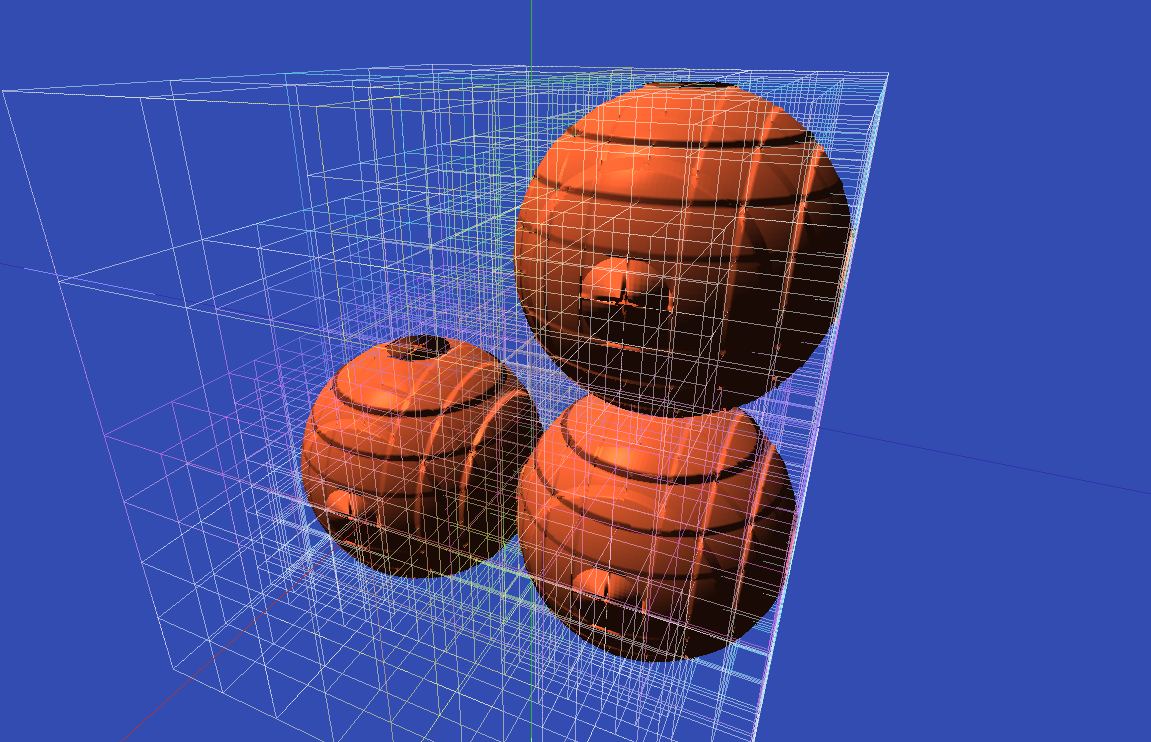
\includegraphics[height=6cm]{marching_artifacts.png}
    \caption{Ray marching artifacts when borders are simple copy of neighboring sdf values.}
    \label{border_artifacts}
\end{figure}

\subsection{Rendering}
Rendering the selected bricks using the vertex shader and geometry shader is straightforward. The real challenge is selecting the bricks for rendering in the \uv{LOD-Occlusion query} pass.
Unfortunately, there was not enough time to implement a~more advanced solution, so for each model, all bricks from a~particular SVO level are submitted for rendering. A~crude and simple LOD method was implemented where the SVO level for a~particular model is selected based on the distance of the model from the camera. This allowed for testing the continuity of the visual quality of the model image when transitioning between different SVO levels.

An interesting aspect of the implementation was the actual ray-marching inside the volume of the rasterized cube. The core algorithm is visualized in the diagram in figure \ref{pipeline_idea}. The linear interpolator of the texture sampler unit is used, so the distance value might be sampled at any point in the cube's interior, creating smooth gradients of distance values in 3D space.

The main challenge was to correctly transform and orient the marched cube and ray with the camera, because the rasterized cube could be anywhere with any orientation depending on the transform matrix of its model.
At the end, the needed transformation of the brick and camera position are pre-computed in previous stages, so that in the actual per-fragment shader, only the fragment position needs to be multiplied with the pre-computed transformation matrix.

The normal on the hit surface is computed as a~gradient on the SDF function using the code described in \cite{Quilez_normals}.
Fragments with missed rays are discarded to make the cube transparent.
The last thing needed to implement for the renderer to be temporarily coherent was correcting the depth buffer value of the fragment, which was done by projecting the hit point into clip space and sampling its depth from homogeneous coordinates.

%%%%%%%%%%%%%%%%%%%%%%%%%%%%%%%%%%%%%%%%%%%%%%%%%%%%%%%%%%%%%%%%%%%%%%%%%%%%%%%%%%%%%%%%

\section{Results}

The final application is able to load a~scene from a~json file consisting of geometries and models. It then evaluates the geometries into the SVO representation described above and renders the models with minimal visual artifacts. It can evaluate and re-render edits of 7 different primitives with additional \uv{rounding} and \uv{blending} properties. Each edit can be placed and rotated in space, as well as each model. On figure \ref{primitives_scene}, there is a~screenshot of a~scene presenting all possible primitives rendered by the program.

\begin{figure}
    \centering
    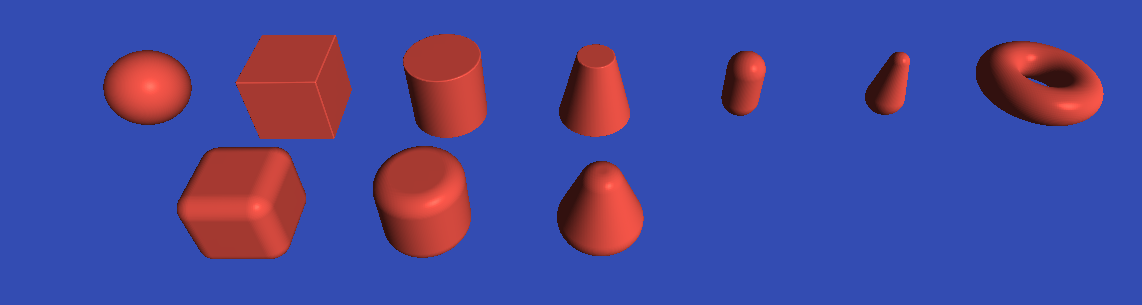
\includegraphics[width=\textwidth]{primitives_scene.png}
    \caption{Sample of all possible shapes.}
    \label{primitives_scene}
\end{figure}
As a~demonstration of better usability, a~scene of a~chess board was modeled using the json representation, as can be seen in figures \ref{chess} and \ref{chess2}.
A test for the evaluator was also implemented by randomly animating individual edits in the geometry and re-evaluating it each frame, as shown in figure \ref{floating}.
\begin{figure}
    \centering
    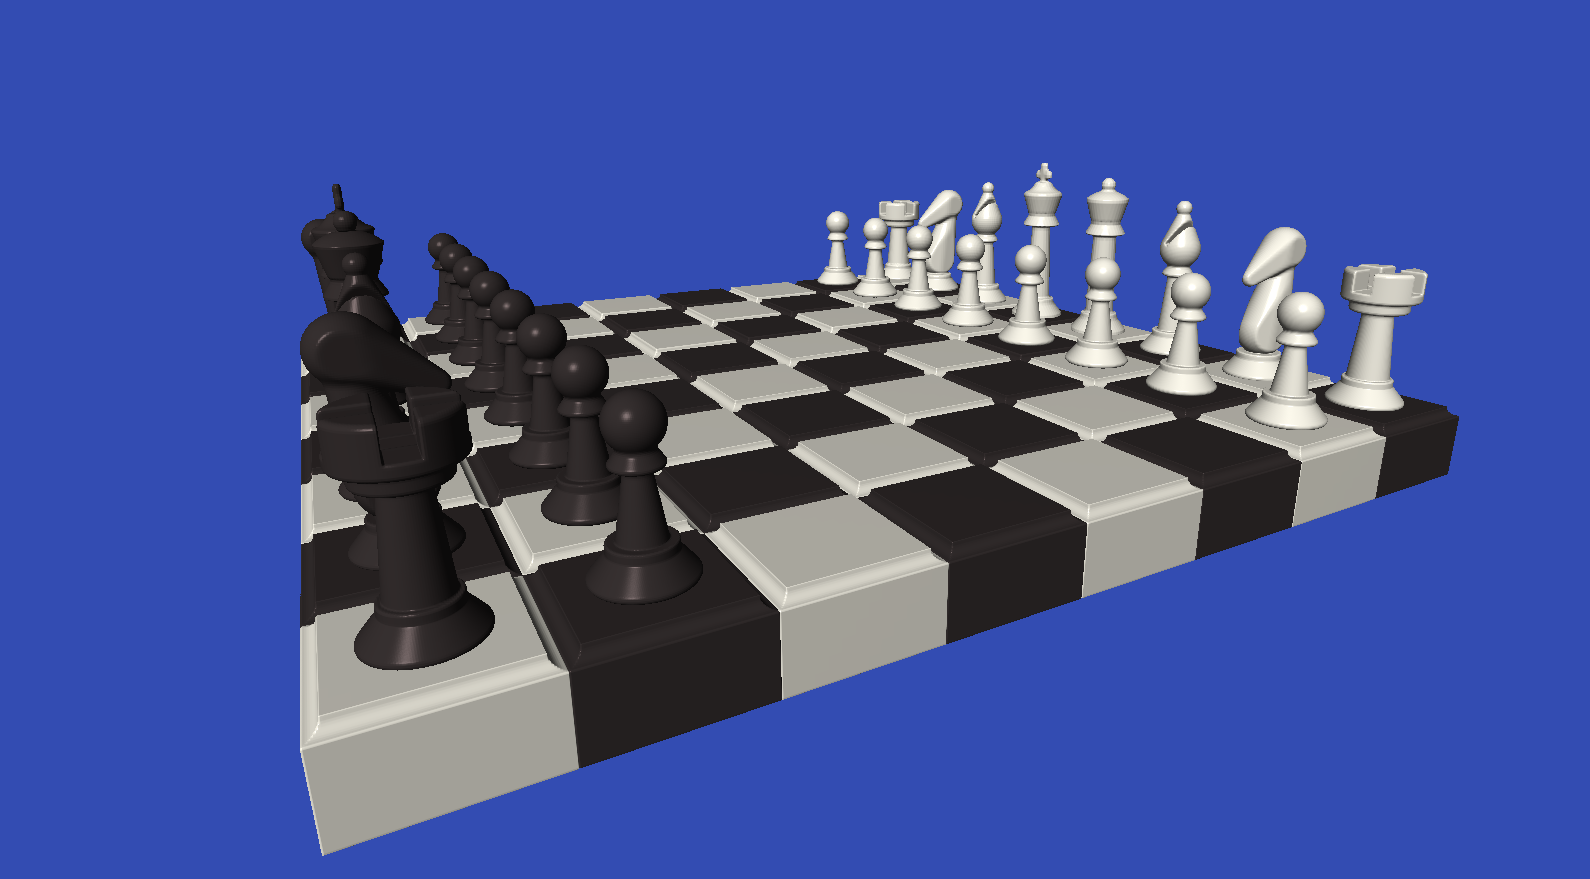
\includegraphics[width=.45\textwidth]{chess.png}
    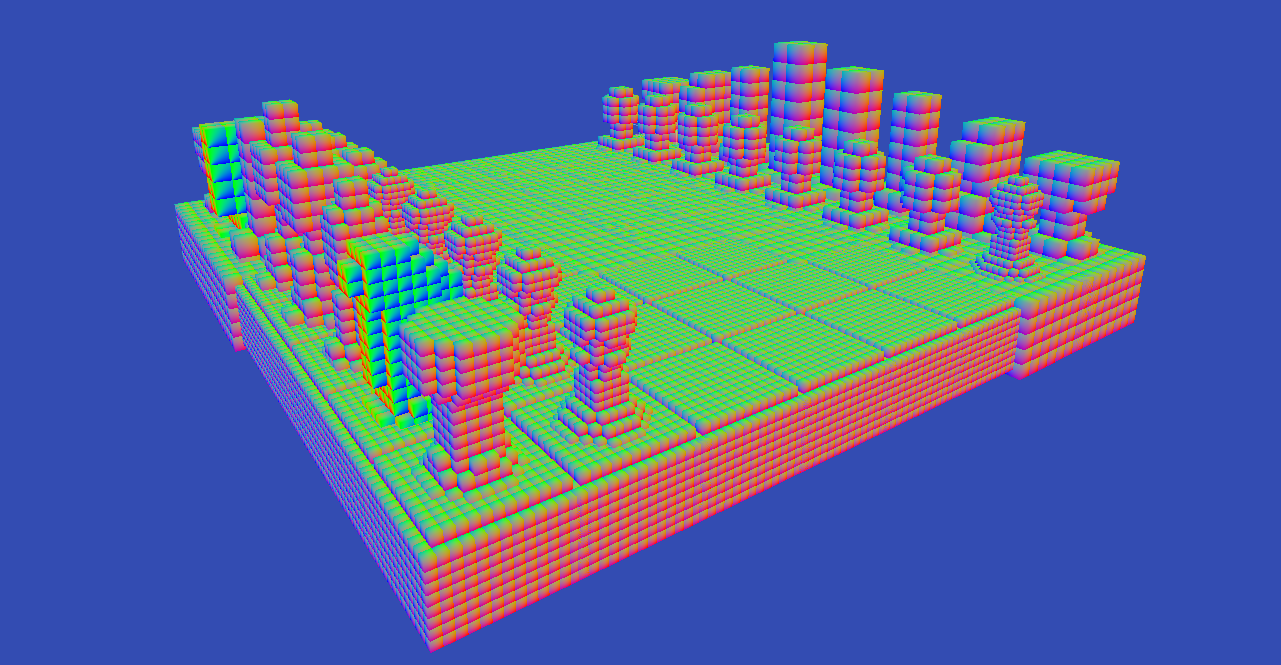
\includegraphics[width=.45\textwidth]{chessBoxes.png}
    \caption{Chess demo scene with custom SDF models. Right - boxes rasterized without ray marching, there can be seen a~different level of the SVO in further models.}
    \label{chess}
\end{figure}
\begin{figure}
    \centering
    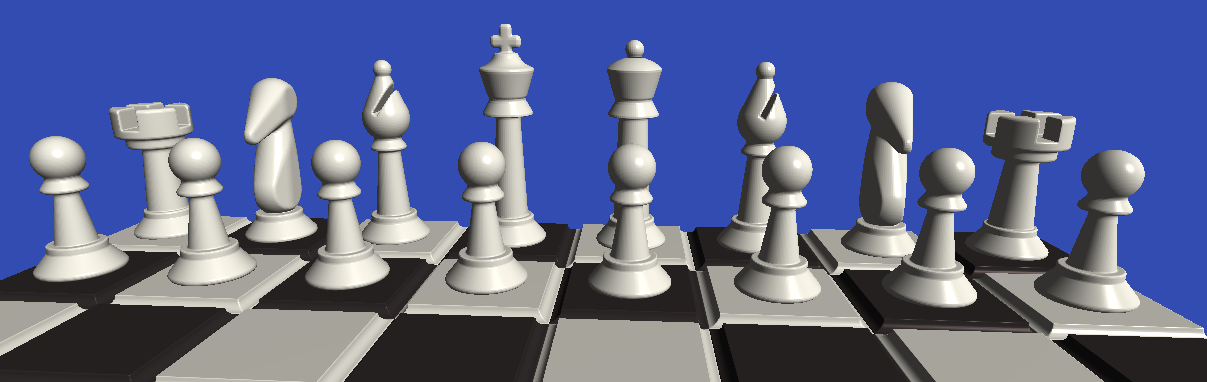
\includegraphics[width=\textwidth]{chess2.png}
    \caption{Detail of SDF models of chess figures.}
    \label{chess2}
\end{figure}
\begin{figure}
    \centering
    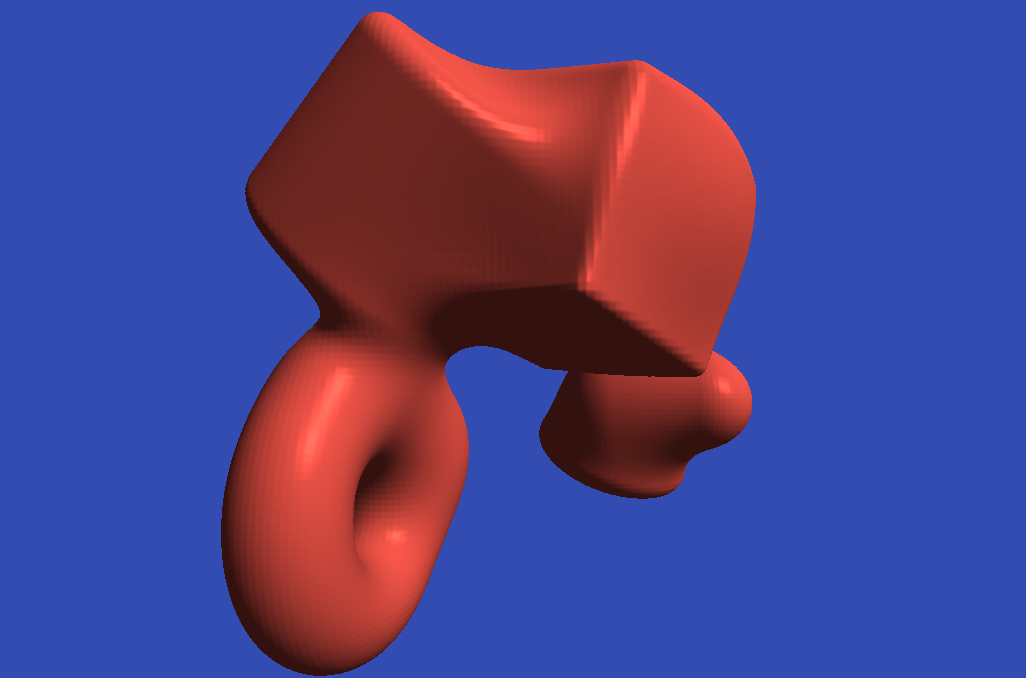
\includegraphics[height=5.5cm]{floating.png}
    \caption{Evaluator real-time test.}
    \label{floating}
\end{figure}

%%%%%%%%%%%%%%%%%%%%%%%%%%%%%%%%%%%%%%%%%%%%%%%%%%%%%%%%%%%%%%%%%%%%%%%%%%%%%%%%%%%%%%%%

\section{Conclusion}

This work has successfully represented a~scene composed of SDF models and rendered it using per-brick rasterization.
The implemented algorithms are not optimal and could be improved.
The stress test showed that the evaluator cannot handle deeper levels of the SVO or a~larger number of primitives in real-time, but this is likely due to the inefficient implementation using the alternation of two programs, an unoptimized implementation of the SDF for primitives, and the lack of a~hierarchical acceleration data structure for the list of primitives.
In the future, there will be a~major refactoring of the entire evaluation process using a~single program and possibly persistent threads to construct the entire SVO in one dispatch.
An acceleration spatial data structure can be implemented for the edit lists.
The actual SDF computation could also be accelerated using efficient max-norms as described in \cite{gokul2003}.
The rendering works well, but more work needs to be done on the actual \uv{LOD-Occlusion Query}, where ideally, the LOD will be per-brick, and only unoccluded and visible bricks will be submitted for rendering.
To enhance the visual quality, there is potential for per-voxel colorization, implementation of shadows, and global illumination models.

\bibliographystyle{alpha}
\begin{flushleft}
    \bibliography{project}
\end{flushleft}

\end{document}
